\chapter{Scheduling}

\epigraph{I wish that I could fly\\
There's danger if I dare to stop and here's the reason why\\
You see I'm overdue\\
I'm in a rabbit stew\\
Can't even say "Good-bye", hello\\
I'm late, I'm late, I'm late\\
No, no, no, no, no, no, no!}{Alice in Wonderland}

CPU Scheduling is the problem of efficiently selecting which process to run on a system's CPU cores.
In a busy system, there will be more ready-to-run processes than there are CPU cores, so the system kernel must evaluate which processes should be scheduled to run and which processes should be executed later.
The system must also decide whether or not it should take a particular process and pause its execution -- along with any associated threads.
The balance comes from stopping processes often enough where you have a responsive computer but infrequently enough where the programs themselves are not spending a lot of cycles context switching.
It is a hard balance it get right.

The additional complexity of multi-threaded and multiple CPU cores are considered a distraction to this initial exposition so are ignored here.
Another gotcha for non-native speakers is the dual meanings of ``Time'': The word ``Time'' can be used in both clock and elapsed duration context.
For example ``The arrival time of the first process was 9:00am.'' and, ``The running time of the algorithm is 3 seconds''.

One clarification that we will make is that our scheduling will mainly deal with short term or cpu scheduling.
That means we will assume that the processes are in memory and ready to go.
The other types of scheduling are long and medium term.
Long term schedulers act as gatekeepers to the processing world.
When a process requests another process to be executed, it can either tell tell the process yes, no, or wait.
The medium term scheduler deals with the caveats of moving a process from the paused state in memory to the paused state on disk when there are too many processes or some process are known not to be used for a significant amount of CPU cycles.
Think about a process that only checks something once an hour.

\section{High Level Scheduler Overview}

Schedulers are pieces of software programs. In fact, you can implement schedulers yourself!
If you are given a list of commands to exec, you can run them with SIGSTOP and SIGCONT.
These are called user space schedulers.
Hadoop and python's celery may do some sort of user space scheduling or deal with the operating system.

At the operating system you generally have this type of flowchart, described in words first below.
Note, please don't memorize all the states.

\begin{enumerate}
\item New is the initial state. A process has just been requested to schedule. All process requests come from fork or clone. At this point the operating system knows it needs to create a new process.
\item A process moves from the new state to the ready. This means any structs in the kernel are allocated an there are only a few low latency steps (by comparison) needed to perform a context process switch. From there it can go into ready suspended or running.
\item Running is the state that we hope most of our processes are in, meaning they are doing useful work. A process could either get pre-empted, blocked, or terminate. Pre-emption brings the process back to the ready state. If a process is blocked, that means it could be waiting on a mutex lock, or it could've called sleep -- either way it willingly gave up control.
\item On the blocked state the operating system can either turn the process ready or it can go into a deeper state called blocked suspended.
\item There are so-called deep slumber states called blocked suspended and blocked ready. You don't need to worry about these.
\end{enumerate}

The reason that we mention this even though you don't need to memorize the transitions is it's important to know that scheduling is much more about the measures below -- in fact the content below is more related to queueing theory than it is to scheduling as a whole.
This means that we will try to pick a scheme that decides when a process should move to the running state, and when it should be moved back to the ready state.
We won't make much mention of how to factor in voluntary blocked states and when to switch to deep slumber states.

\section{Measurements}

Scheduling effects the performance of the system, specifically the \emph{latency} and \emph{throughput} of the system.
The throughput might be measured by a system value, for example the I/O throughput - the number of bits written per second, or number of small processes that can complete per unit time.
The latency might be measured by the response time -- elapse time before a process can start to send a response -- or wait time or turnaround time --the elapsed time to complete a task.
Different schedulers offer different optimization trade-offs that may or may not be appropriate to desired use.
There is no optimal scheduler for all possible environments and goals.
For example `shortest-job-first' will minimize total wait time across all jobs but in interactive (UI) environments it would be preferable to minimize response time at the expense of some throughput, while FCFS seems intuitively fair and easy to implement but suffers from the Convoy Effect.
Arrival time is the time at which a process first arrives at the ready queue, and is ready to start executing.
If a CPU is idle, the arrival time would also be the starting time of execution.

\subsection{What is preemption?}

Without preemption processes will run until they are unable to utilize the CPU any further.
For example the following conditions would remove a process from the CPU and the CPU would be available to be scheduled for other processes.
The process terminates due to a signal, is blocked waiting for concurrency primitive, or exits normally.
Thus once a process is scheduled it will continue even if another process with a high priority appears on the ready queue.

With preemption, the existing processes may be removed immediately if a more preferable process is added to the ready queue.
For example, suppose at t=0 with a Shortest Job First scheduler there are two processes (P1 P2) with 10 and 20 ms execution times.
P1 is scheduled.
P1 immediately creates a new process P3, with execution time of 5 ms, which is added to the ready queue.
Without preemption, P3 will run 10ms later (after P1 has completed).
With preemption, P1 will be immediately evicted from the CPU and instead placed back in the ready queue, and P3 will be executed instead by the CPU.

Any scheduler that doesn't use some form of pre-emption can result in starvation because earlier processes may never be scheduled to run (assigned a CPU).
For example with SJF, longer jobs may never be scheduled if the system continues to have many short jobs to schedule.
It all depends on the \href{https://en.wikipedia.org/wiki/Scheduling_(computing)\#Types_of_operating_system_schedulers}{type of scheduler}.

\subsection{Why might a process (or thread) be placed on the ready queue?}

A process is placed on the ready queue when it is able to use a CPU. Some examples include:

\begin{itemize}
  \tightlist
\item A process was blocked waiting for a \keyword{read} from storage or socket to complete and data is now available.
\item A new process has been created and is ready to start.
\item A process thread was blocked on a synchronization primitive (condition variable, semaphore, mutex lock) but is now able to continue.
\item A process is blocked waiting for a system call to complete but a signal has been delivered and the signal handler needs to run.
\end{itemize}

\section{Measures of Efficiency}

First some definitions

\begin{enumerate}
  \item \keyword{start\_time} is the wall-clock start time of the process (CPU starts working on it)
  \item \keyword{end\_time} is the end wall-clock of the process (CPU finishes the process)
  \item \keyword{run\_time} is the total amount of CPU time required
  \item \keyword{arrival\_time} is the time the process enters the scheduler (CPU may not start working on it)
\end{enumerate}

Here are measures of efficiency and their mathematical equations

\begin{enumerate}
\item \keyword{Turnaround Time} is the total time from when you the process arrives to when it ends.
  \keyword{end\_time - arrival\_time}
  \item \keyword{Response Time} is the total latency (time) that it takes from when the process arrives to when the CPU actually starts working on it.
    \keyword{start\_time - arrival\_time}
  \item \keyword{Wait Time} is the \emph{total} wait time or the total time that a process is on the ready queue.
    A common mistake is to believe it is only the initial waiting time in the ready queue.
    If a CPU intensive process with no I/O takes 7 minutes of CPU time to complete but required 9 minutes of wall-clock time to complete we can conclude that it was placed on the ready-queue for 2 minutes.
    For those 2 minutes, the process was ready to run but had no CPU assigned.
    It does not matter when the job was waiting, the wait time is 2 minutes.
    \keyword{end\_time - arrival\_time - run\_time}

\end{enumerate}

\subsection{Convoy Effect}

The convoy effect is when a process takes up a lot of the CPU time, leaving all other process with potentially smaller resource needs following like a Convoy Behind them.

Suppose the CPU is currently assigned to a CPU intensive task and there is a set of I/O intensive processes that are in the ready queue.
These processes require just a tiny amount of CPU time but they are unable to proceed because they are waiting for the CPU-intensive task to be removed from the processor.
These processes are starved until the the CPU bound process releases the CPU.
But, the CPU will rarely be released.
For example in the case of a FCFS scheduler, we must wait until the processes is blocked due to an I/O request.
The I/O intensive processes can now finally satisfy their CPU needs, which they can do quickly because their CPU needs are small and the CPU is assigned back to the CPU-intensive process again.
Thus the I/O performance of the whole system suffers through an indirect effect of starvation of CPU needs of all processes.

This effect is usually discussed in the context of FCFS scheduler, however a round robin scheduler can also exhibit the Convoy effect for long time-quanta.

\subsection{Extra: Linux Scheduling}

As of February 2016, Linux by default uses the \emph{Completely Fair Scheduler} for CPU scheduling and the Budget Fair Scheduling ``BFQ'' for I/O scheduling. Appropriate scheduling can have a significant impact on throughput and latency. Latency is particularly important for interactive and soft-real time applications such as audio and video streaming. See the discussion and comparative benchmarks \href{https://lkml.org/lkml/2014/5/27/314}{here} for more information.

Here is how the CFS schedules

\begin{itemize}
\tightlist
\item
  The CPU creates a Red-Black tree with the processes virtual runtime (runtime / nice\_value) and sleeper fairness flag (if the process is waiting on something give it the CPU when it is done waiting).
\item
  (Nice values are the kernel's way of giving priority to certain processes, the lower nice value the higher priority)
\item
  The kernel chooses the lowest one based on this metric and schedules that process to run next, taking it off the queue. Since the red-black tree is self balancing this operation is guaranteed \(O(log(n))\) (selecting the min process is the same runtime)
\end{itemize}

Although it is called the Fair Scheduler there are a fair bit of problems.

\begin{itemize}
\tightlist
\item
  Groups of processes that are scheduled may have imbalanced loads so the scheduler roughly distributes the load. When another CPU gets free it can only look at the average load of a group schedule not the individual cores. So the free CPU may not take the work from a CPU that is burning so long as the average is fine.
\item
  If a group of processes is running on non-adjacent cores then there is a bug. If the two cores are more than a hop away, the load balancing algorithm won't even consider that core. Meaning if a CPU is free and a CPU that is doing more work is more than a hop away, it won't take the work (may have been patched).
\item
  After a thread goes to sleep on a subset of cores, when it wakes up it can only be scheduled on the cores that it was sleeping on. If those cores are now busy, the thread will have to wait on them, wasting opportunities to use other idle cores.
\item
  To read more on the problems of the Fair Scheduler, read \href{https://blog.acolyer.org/2016/04/26/the-linux-scheduler-a-decade-of-wasted-cores}{here}.
\end{itemize}

\section{Scheduling Algorithms}

Unless otherwised stated

\begin{enumerate}
\item Process 1: Runtime 1000ms
\item Process 2: Runtime 2000ms
\item Process 3: Runtime 3000ms
\item Process 4: Runtime 4000ms
\item Process 5: Runtime 5000ms
\end{enumerate}

\subsection{Shortest Job First (SJF)}

\begin{figure}[htbp]
\centering
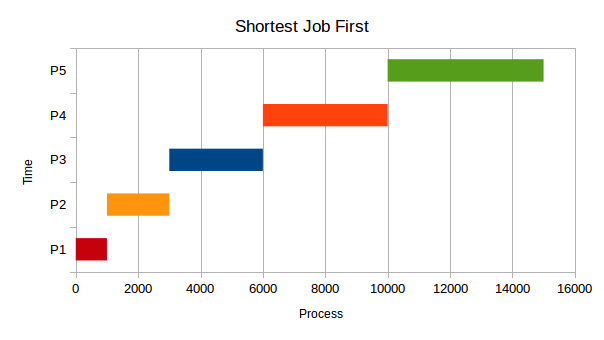
\includegraphics[width=\textwidth]{scheduling/images/sjf.png}
\caption{Shortest job first scheduling}
\end{figure}

\begin{itemize}
\tightlist
\item
  P1 Arrival: 0ms
\item
  P2 Arrival: 0ms
\item
  P3 Arrival: 0ms
\item
  P4 Arrival: 0ms
\item
  P5 Arrival: 0ms
\end{itemize}

The processes all arrive at the start and the scheduler schedules the job with the shortest total CPU time.
The glaring problem is that this scheduler needs to know how long this program will run over time before it ran the program.

Technical Note: A realistic SJF implementation would not use the total execution time of the process but the burst time.
The total CPU time including future computational execution before the process will no longer be ready to run.
The expected burst time can be estimated by using an exponentially decaying weighted rolling average based on the previous burst time \todo{Citation Needed}.
For this exposition we will simplify this discussion to use the total running time of the process as a proxy for the burst time.

\textbf{Advantages}

\begin{enumerate}
  \item Shorter jobs tend to get run first
  \item On average wait times and response times are down
\end{enumerate}

\textbf{Disadvantages}
\begin{enumerate}
  \item Needs algorithm to be omniscient
  \item Need to estimate the burstiness of a process which is harder than let's say a computer network
\end{enumerate}

\subsection{Preemptive Shortest Job First (PSJF)}

Preemptive shortest job first is like shortest job first but if a new job comes in with a shorter runtime than the total runtime of the current job, it is run instead.
If it is equal like our example our algorithm can choose.
The scheduler uses the \emph{total} runtime of the process.
If you want the shortest \emph{remaining} time left, that is a variant of PSJF called Shortest Remaining Time First (SRTF).

\begin{figure}[htbp]
\centering
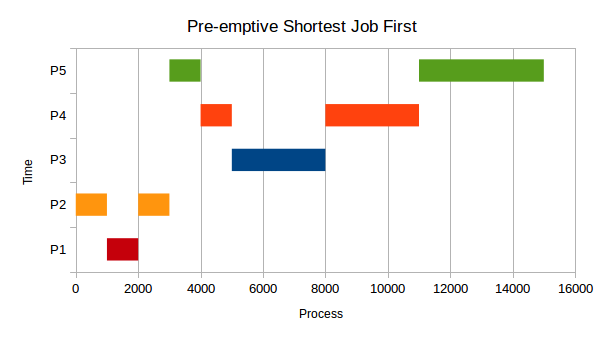
\includegraphics[width=\textwidth]{scheduling/images/psjf.png}
\caption{Preemptive Shortest Job First scheduling}
\end{figure}

\begin{itemize}
\tightlist
\item
  P2 at 0ms
\item
  P1 at 1000ms
\item
  P5 at 3000ms
\item
  P4 at 4000ms
\item
  P3 at 5000ms
\end{itemize}

Here's what our algorithm does.
It runs P2 because it is the only thing to run.
Then P1 comes in at 1000ms, P2 runs for 2000ms, so our scheduler preemptively stops P2, and let's P1 run all the way through.
This is completely up to the algorithm because the times are equal.
Then, P5 Comes in -- since there are no processes running, the scheduler will run process 5.
P4 comes in, and since the runtimes are equal P5, the scheduler stops P5 and runs P4.
Finally P3 comes in, preempts P4, and runs to completion.
Then P4 runs, then P5 runs.

\textbf{Advantages}

\begin{enumerate}
  \item Ensures shorter jobs get run first
\end{enumerate}

\textbf{Disadvantages}

\begin{enumerate}
  \item Need to know the runtime again
  \item Context switching and jobs can get interrupted
\end{enumerate}

\subsection{First Come First Served (FCFS)}

\begin{figure}[htbp]
\centering
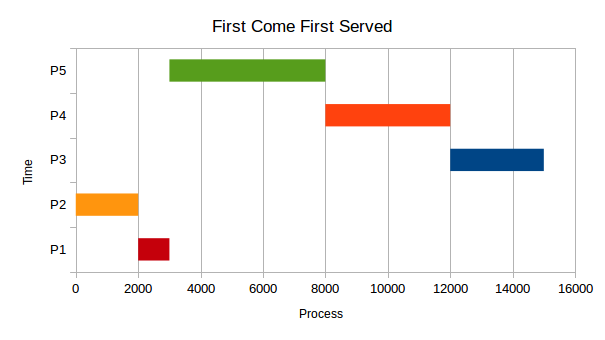
\includegraphics[width=\textwidth]{scheduling/images/fcfs.png}
\caption{First come first serve scheduling}
\end{figure}

\begin{itemize}
\tightlist
\item
  P2 at 0ms
\item
  P1 at 1000ms
\item
  P5 at 3000ms
\item
  P4 at 4000ms
\item
  P3 at 5000ms
\end{itemize}

Processes are scheduled in the order of arrival.
One advantage of FCFS is that scheduling algorithm is simple
The ready queue is a just a FIFO (first in first out) queue.
FCFS suffers from the Convoy effect.
Here P2 Arrives, then P1 arrives, then P5, then P4, then P3. You can see the convoy effect for P5.

\textbf{Advantages}

\begin{itemize}
\item Simple algorithm and implementation
\item Context switches infrequent when there are long running processes
\item No starvation if all processes are guaranteed to terminate
\end{itemize}

\textbf{Disadvantages}
\begin{itemize}
\item Simple algorithm and implementation
\item Context switches infrequent when there are long running processes

\end{itemize}

\subsection{Round Robin (RR)}

Processes are scheduled in order of their arrival in the ready queue.
However after a small time step, a running process will be forcibly removed from the running state and placed back on the ready queue.
This ensures that a long-running process can not starve all other processes from running.
The maximum amount of time that a process can execute before being returned to the ready queue is called the time quanta.
As the time quanta goes to infinity, round robin will be equivalent to FCFS.

\begin{figure}[htbp]
\centering
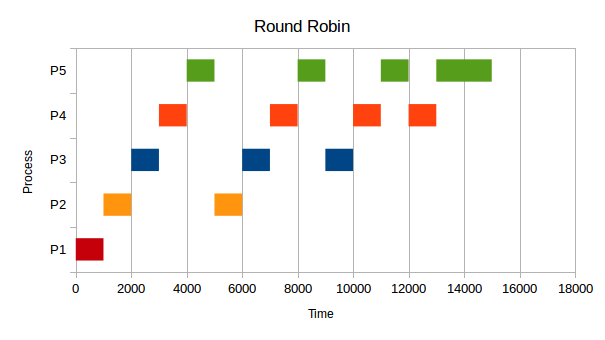
\includegraphics[width=\textwidth]{scheduling/images/rr.png}
\caption{Round Robin Scheduling}
\end{figure}

\begin{itemize}
\tightlist
\item
  P1 Arrival: 0ms
\item
  P2 Arrival: 0ms
\item
  P3 Arrival: 0ms
\item
  P4 Arrival: 0ms
\item
  P5 Arrival: 0ms
\end{itemize}

Quantum = 1000ms

Here all processes arrive at the same time.
P1 is run for 1 quantum and is finished.
P2 for one quantum; then, it is stopped for P3.
After all other processes run for a quantum we cycle back to P2 until all the processes are finished.

\textbf{Advantages}

\begin{enumerate}
  \item Ensures some notion of fairness
\end{enumerate}

\textbf{Disadvantages}

\begin{enumerate}
  \item Large number of processes = Lots of switching
\end{enumerate}

\subsection{Priority}

Processes are scheduled in the order of priority value.
For example, a navigation process might be more important to execute than a logging process.

\section{Scheduling Conceptually}

Okay so we've given you a bunch of tools, but if your co-worker came up to you now and asked you what scheduling algorithm to use, you wouldn't really know what to say.
So let's think about scheduling algorithms at a high level and break them down by their times.
We will be evaluating this in the context of a random process timing, meaning that each process takes a random but fininte amount of time to finish.

Just a refresher, here are the terms.

\begin{tabular}{|c|c|}
  Concept & Meaning \\ \hline
  Start time & The time the scheduler first started work \\
  End time & When the scheduler finished the process \\
  Arrival time & When the job first arrived at the scheduler \\
  Run time & How long does the process take to run if there is no pre-emption
\end{tabular}

And here are the measures we are trying to optimize.

\begin{tabular}{|c|c|}
  Measure & Formula \\ \hline
  Response Time & Start time minus Arrival time\\
  Turnaround time & End time minus Arrival time\\
  Wait time & End time minus Arrival time minus Run time \\
\end{tabular}

Other discussions about different use cases will be discussed after.
To make any mathematical arguments either, let the maximum amount of time that a process run be equal to $S$.
We will also assume that there are a finite number of processes running at any given time $c$.

We will also be include mathematical results in this section \textbf{These results are not essential to going through the course, but they will let you understand how we can compare different distributions}.
Some more mathematically oriented students may like the reasoning behind our comparisons.
Here are some concepts from queueing theory that you'll need to know that will help simplify the theories.

\begin{enumerate}
\item Queueing theory involves a random variable controlling the interarrival time -- or the time between two different processes arriving.
  We won't name this random variable, but we will assume that (1) it has a mean of $\lambda$ and (2) it is distributed as a poisson random variable.
  This means the probability of getting a process $t$ units after getting another process is $\lambda^t * \frac{\exp(-\lambda)}{t!}$ where $t!$ can be approximated by the gamma function when dealing with real values.
\item We will be denoting the service time $S$, and deriving the waiting time $W$, and the response time $R$; more specifically the expected values of all of those variables $E[S]$ deriving turnaround time is simply $S + W$.
  For clarity we will introduce another variable $N$ that is the number of people currently in the queue.
  A famous result in queueing theory is Little's Law which states $E[N] = \lambda E[W]$ meaning that the number of people waiting is the arrival rate times the expected waiting time (assuming the queue is in a steady state).
\item We won't make many assumptions about how much time it'll take to run each process except that it will take a finite amount of time -- otherwise this gets almost impossible to evaluate.
We will however denote two variables that $\frac{1}{\mu}$ is the mean of the waiting time and that the coefficient of variation $C$ is defined as $C^2 = \frac{var(S)}{E[S]^2}$ to help us control for processes that take a while to finish.
An important note is that when $C > 1$ we say that the running times of the process are variadic. We will note below that this rockets up the wait and response times for FCFS quadratically.
\item $\rho = \frac{\lambda}{\mu} < 1$ Otherwise our queue would become infinitely long
\item We will assume that there is one processor. This is known as a M/G/1 queue in queueing theory.
\item We'll leave the service time as an expectation $S$ otherwise we may run into over-simplifications with the algebra.
  Plus it is easier to compare different queueing disciplines with a common factor of service time.
\end{enumerate}

\subsection{First Come First Served}

All results are from Jorma Virtamo's lectures on the matter \cite{virtamo}

\begin{enumerate}
\item The first is expected waiting time.
  \[
  E[W] = \frac{(1 + C^2)}{2}\frac{\rho}{(1 - \rho)} * E[S]
  \]

  What does this say? When given as $\rho \rightarrow 1$ or the mean job arrival rate equals the mean job processing rate, then the wait times get really long.
  In addition, as the variance of the job increases, the wait times go up.

\item Next is the expected response time

  \[
  E[R] = E[N] * E[S] = \lambda * E[W] * E[S]
  \]
  The response time is simple to calculate, it is just the expected number of people ahead of the process in the queue times the expected time to service each of those processes.
  From Little's law above, we can substitute that for this. Since we already know the value of the waiting time, we can reason about the response time as well.
\item A discussion of the results is shows something very cool discovered by Conway and Al \cite{conway1967theory}.
  Any scheduling discipline that isn't pre-emptive and doesn't take into account the run time of the process or a priority will have the same wait, response, and turnaround time.
  We will often use this as a baseline.
\end{enumerate}

\subsection{Round Robin or Processor Sharing}

It is really hard to analyze round robin from a probabilistic sense because it is so state based.
The next job that you work on requires you to remember the previous jobs.
Queueing theory developers have made an assumption that the time quanta is roughly zero -- ignoring context switching and the like.
This leads way into processor sharing.
Many different tasks can get worked on at the same time but experience a slowdown.
All of these proofs will be adapted from Harchol-Balter's book \cite{harchol2013performance}.
I highly recommend checking out the books if you are interested.
The proofs are intuitive for people who don't have a background in queueing theory.

\begin{enumerate}
  \item Before we jump to the answer let's reason about this.
    With our new-found abstraction, we essentially have a FCFS queue where we are going to be working on each job a little slower than before.
    Since we are never not working on a job

    \[
    E[W] = 0
    \]

  Under a non-strict analysis of processor sharing though, the amount of time that you wait is best approximated by the amount of times you need to wait.
  You'll need $\frac{E[S]}{Q}$ service periods where $Q$ is the quanta, and you'll need about $E[N] * Q$ time in between those periods.
  Leading to an average time of
  \[
  E[W] = E[S] * E[N]
  \]

  The reason this proof is not rigorous and not accepted is because we can't assume that there will always be $E[N] * Q$ time on average in between cycles because it depends on the state of the system.
  This means we need to factor in various variations in processing delay.
  We also can't use Little's law in this case because there is no real steady state of the system (otherwise we'd be able to prove some weird things)

  One thing that is interesting is that we don't have to worry about the convoy effect or any new processes coming in.
  The total wait time remains bounded by the number of people in the queue.
  For those of you familiar with tail inequalities since processes arrive according to a poinsson distribution, the probability that we'll get many processes drops off exponentially due to chernoff bounds (all arrivals are independent of other arrivals).
  Meaning roughly we can assume low variance on the number of processes.
  As long as the service time is reasonable on average, the wait time will be too.

\item The expected response time is
  \[
  E[R] = 0
  \]

  Under strict processor sharing it is 0 because all jobs are worked on.
  In practice however, the response time is.
  \[
  E[R] = E[N] * Q
  \]

  Where $Q$ is the quanta.
  Using Little's Law again, we can find out that
  \[
  E[R] = \lambda E[W] * Q
  \]
\item One variable that is different is the amount of service time let the service time for processor sharing be defined as $S_{PS}$.
  The slowdown is $E[S_{PS}] = \frac{E[S]}{1 - \rho}$
  Which means as the mean arrival rate equals the mean processing time, then the jobs will take asymptotically as long to finish.
  In the non-strict analyis of processor sharing, we assume that
  \[
    E[S_{RR}] = E[S] + Q * \epsilon, \epsilon > 0
  \]
    $\epsilon$ is the amount of time a context switch takes.

\item That naturally leads to the comparison, what is better?
  The response time is roughly the same comparing the non-strict versions, the wait time is roughly the same, but notice that nothing about the variation of the jobs is put in.
  That's because RR doesn't have to deal with the convoy effect and any variances associated, otherwise FCFS is faster in a strict sense.
  It also takes more times for the jobs to finish, but the overall turnaround time is lower under high variance loads.
\end{enumerate}

\subsection{Non Pre-emptive Priority}

We will introduce the notation that there are $k$ different priorities and $\rho_i > 0$ is the average load contribution for priority $i$ We are constrained by $\sum\limits_{i=0}^k \rho_i = \rho$.
We will also denote $\rho(x) = \sum\limits_{i=0}^x \rho_i$ which is the load contribution for all higher and similar priority processes to $x$.
The last bit of notation is that we will assume that the probability of getting a process of priority $i$ is $p_i$ and naturally $\sum\limits_{j=0}^k p_j = 1$
 
\begin{enumerate}
\item If $E[W_i]$ is the wait time for priority $i$,
  \[
  E[W_x] = \frac{(1 + C)}{2}\frac{\rho}{(1 - \rho(x))*( 1 - \rho(x-1))} * E[S_i]
  \]
    The full derivation is as always in the book.
    A more useful inequality is that.

    \[
    E[W_x] \leq \frac{1 + C}{2}* \frac{\rho}{(1 - \rho(x))^2} * E[S_i]
    \]
    because the addition of $\rho_x$ can only increase the sum, decrease the denominator or increase the overal function.
  This means that if one is priority 0, then a process only need to wait for the other P0 processes which there should be $\rho C/ (1 - \rho_0)$ P0 processes arrived before to process in FCFS order.
  Then the next priority has to wait for all the others and so on and so forth.

  The expected overall wait time is now

  \[
      E[W] = \sum\limits_{i=0}^k E[W_i] * p_i
  \]

  Now that we have notational soup, let's factor out the important terms.

  \[
      \sum\limits_{i=0}^k \frac{p_i}{(1-\rho(i))^2}
  \]

  Which we compare with FCFS' model of

  \[
      \frac{1}{1-\rho}
  \]

  In words -- you can work this out with experiementing distributions -- if you have a lot of low priority processes who don't contribute a lot to the average load, your average wait time becomes much lower.

\item The average per process response time is

  \[
  E[R_i] = \sum\limits_{j = 0}^i E[N_j] * E[S_j]
  \]

  Which simply says that you need to wait for all jobs with a higher priority and the same to go before you can go.
  Imagine a series of FCFS queues which you need to wait your turn.
  Using Little's Law for different colored jobs and the formula above we can simplify this

  \[
      E[R_i] = \sum\limits_{j=0}^i \lambda_j E[W_j] * E[S_j]
  \]

  And we can find the average response time by looking at the distribution of jobs

  \[
      E[R] = \sum\limits_{i=0}^k p_i [\sum\limits_{j=0}^k \lambda_j E[W_j] * E[S_j] ]
  \]

  Meaning that we are tied to wait times and service times of all other processes.
  If we break down this equation, we see again if we have a lot of high priority jobs that don't contribute a lot to the load then our entire sum goes down.
  We won't make too many assumptions about the service time for a job because that would interfere with our analysis from FCFS where we left it as an expression.

  \item As for a comparison with FCFS in the average case, it usually does better assuming that we have a smooth probability distribution -- i.e. the probability of getting any particular priority is zero.
  This is because in all of our formulas, we still have some probability mass to put on lower priority processes, bringing the expectation down.
  This statement doesn't hold for all smooth distributions but for most real-world smoothed distributions (which tend to be smooth) they do.

\item This isn't even to mention the idea of utility.
  Utility means that if we gain an amount of happiness by having certain jobs finish, priority and pre-emptive priority maximize that while balancing out other measures of efficiency.
\end{enumerate}


\subsection{Shortest Job First}
This is a wonderful reduction to the priority.
Instead of having discrete priorities, we'll introduce that a process that takes $S_t$ time to get serviced.
$T$ is the maximum amount of time a process can run for, our processes cannot run infinitely long.
That means the following definitions hold, overriding the previous definitions in priority

\begin{enumerate}
\item Let
  \[
  \rho(x) = \int_0^x \rho_u du
  \]
  Be the average load contribution up to this point.
\item
  \[
  \int_0^k p_u du = 1
  \] Probability constraint.
\item Etc, replace all the summations above with integrals
\item The only notational difference is we don't have to make any assumptions about the service times of the jobs because they are denoted by service times subscript, all other analyses are the same.
  \item This means if you want low wait times on average compared to FCFS, your distribution needs to be right skewed.
\end{enumerate}

\subsection{Pre-emptive Priority}

We will describe priority and sjf's pre-emptive version in the same section because it is essentially the same as we've shown above.
We'll use the same notation as before.
We will also introduce an additional term $C_i$ which denotes the variation among a particular class

\[
    C_i = \frac{var(S_i)}{E[S_i]}
\]

\begin{enumerate}
\item Response Time. Just a head's up, this isn't going to be pretty.
  \[
  E[R_i] = \frac{\sum\limits_{j=0}^i\frac{(1 + C_j)}{2}}{(1 - \rho(x))*( 1 - \rho(x-1))} * E[S_i]
  \]

  If this looks familiar it should.
  This is the average wait time in the non-pre-emptive case with a small change. Instead of using the variance of the entire distribution, we are looking at the variance of each job coming in.
  The whole response times are

  \[
     E[R] = \sum\limits_{i = 0}^k p_i * E[R_i]
  \]

  If lower priorities jobs come in at a higher service time variance, that means our average response times could go down, but not if they make up most of the jobs that come in.
  Think of the extreme cases.
  If 99\% of jobs are high priority jobs and the rest make up the other percent, then the other jobs will get frequently interrupted, but high priority jobs will make up most of the jobs, so the expectation is still low.
  The other extreme is if one percent of jobs are high priority and they come in a very low variance.
  That means the chances us of the system getting a really high priority jobs that will take a long time is low, thus making our response times lower on average.
  We only run into trouble if high priority jobs make up a non-negligable amount, and they have a high variance in service times.
  This brings down response times as well as wait times.

\item Waiting Time
  \[
  E[W_i] = E[R_i] + \frac{E[S_i]}{1 - \rho(i)}
  \]

  Taking the expectation among all processes we get

  \[
  E[W] = \sum\limits_{i = 0}^k p_i (E[R_i] + \frac{E[S_i]}{1 - \rho(i)})
  \]

  We can simplify to

  \[
  E[W] = E[R] + \sum\limits_{i=0}^k \frac{E[S_i]p_i}{(1 - \rho(i))}
  \]

  Which means that we incur the same cost on response time and then we have to suffer an additional cost based on what the probabilities are of lower priority jobs coming in and taking this job out.
  That is what we call the average interruption time.
  This follows the same laws as before.
  Since we have a variadic, pyramid summation if we have a lot of jobs with small service times then the wait time goes down for both additive pieces.
  It can be analytically shown that this is better given certain probability distributions.
  For example, try with the uniform versus FCFS or the non pre-emptive version.
  What happens?
  As always the proof is left to the reader.

\item Turnaround Time is the same formula $E[T] = E[S] + E[W]$. This means that given a distribution of jobs that has either low waiting time as described above, we will get low turnaround time -- we can't really control the distribution of service times.
\end{enumerate}

\subsection{Pre-emptive Shortest Job First}

Unforutnately we can't use the same trick as before because an infinitesimal point doesn't have a well controlled variance.
You can imagine the comparisons though as the same as the previous section.

\section{Topics}

\begin{itemize}
\tightlist
\item
  Scheduling Algorithms
\item
  Measures of Efficiency
\end{itemize}

\section{Questions}

\begin{itemize}
\tightlist
\item
  What is scheduling?
\item
  What is turnaround time? Response Time? Wait time?
\item
  What is the convoy effect?
\item
  Which algorithms have the best turnaround/response/wait time on average
\end{itemize}

\bibliographystyle{plainnat}
\bibliography{scheduling/scheduling}
